\section{Theoretical Analysis} \label{section:theo}


\par In this section, a theoretical analysis of the circuit was conducted. In the introduction, we can see the analysed circuit.

First of all, we got to keep in mind that our circuit is divided in two different stages. The first one corresponds to the gain stage with a NPN transistor and the second is the output stage with a PNP transistor. Both the components and their functions will be described in Theoretical and Simulation Analysis as well as the goal of each stage.

\subsection{Gain Stage}
This stage is responsible for the signal amplification which means it has to have a high gain. It also needs to have a high input voltage to avoid signal losses. In order to analyse this stage we need to study both operating point and incremental analysis.
First,we compute a simple analysis of the circuit by KVL and KCL. This way we obtain $Z_{i1}=R_B||r_{\pi 1}$ and $Z_{o1}=r_{o1}||R_c$. It is important to note that for low frequencies capacitors behave like open circuits and for high frequencys like short circuits.

To analyse the incremental response we have to create a model of the transistor (and the rest of the gain stage) similar to Fig.2. Studying the circuit we get $v_{o1}=-g_m * (r_o||R_c) * v_{\pi}$ and $v_{\pi}= \frac{R_B||r_{\pi 1}}{R_B||r_{\pi 1}+R_s} * v_s $ which lead us to $A_{v1} = \frac{v_{o1}}{v_s} = -g_m * (r_o||R_c)*\frac{R_B||r_{\pi 1}}{R_B||r_{\pi 1}+R_s}$.


\begin{figure}[h] \centering
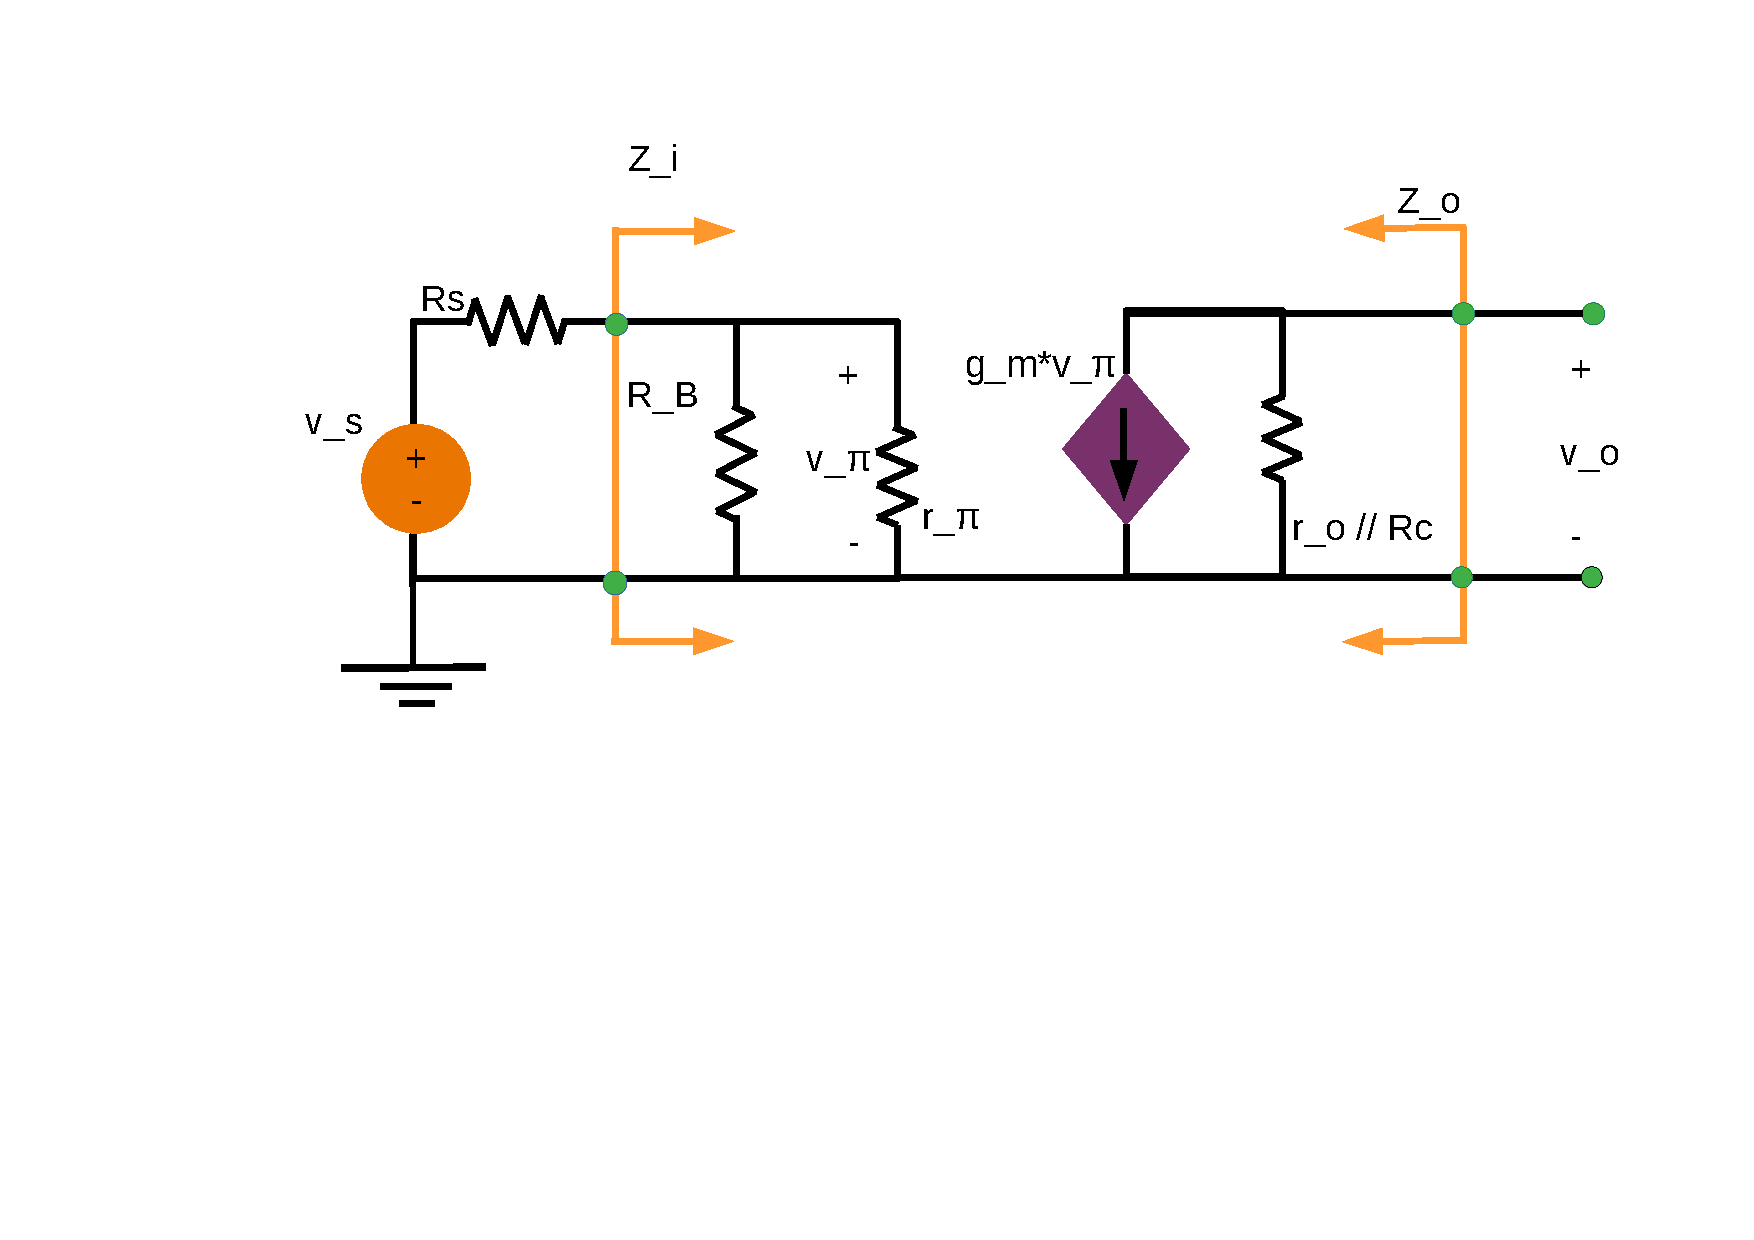
\includegraphics[width=0.8\linewidth]{Incremental_Gain.pdf}
\caption{Model for the gain stage incremental analysis}
\label{sdf}
\end{figure}

\subsection{Output Stage}

However $Z_{o1}$ is too high so we need a second stage to achieve a lower $Z_{o}$. Due to the big difference between the $Z_{o1}$ we can be positive that no voltage signal will be lost.
For the DC response of the output stage, we follow the same logic of the gain stage and we easily get $Z_{i2}=\frac{(g_{m2}+g_{\pi 2}+g_{o2}+g_{E2})}{g_{\pi 2}(g_{\pi 2}+g_{o2}+g_{e2})}$ and $Z_{o2}= \frac{1}{(g_{m2}+g_{\pi2}+g_{o2}+g_{E2})}$. On the other hand, to get the incremental response we have to create another model like Fig.3. Using nodal analysis we end up with $A_{v2} = \frac{v_{o2}}{v_{i2}} = \frac{g_{\pi} + g_{m2} }{g_{\pi 2}+g_{z2}+g_{o2}+g_{m2}}$ for the gain.



\begin{figure}[h] \centering
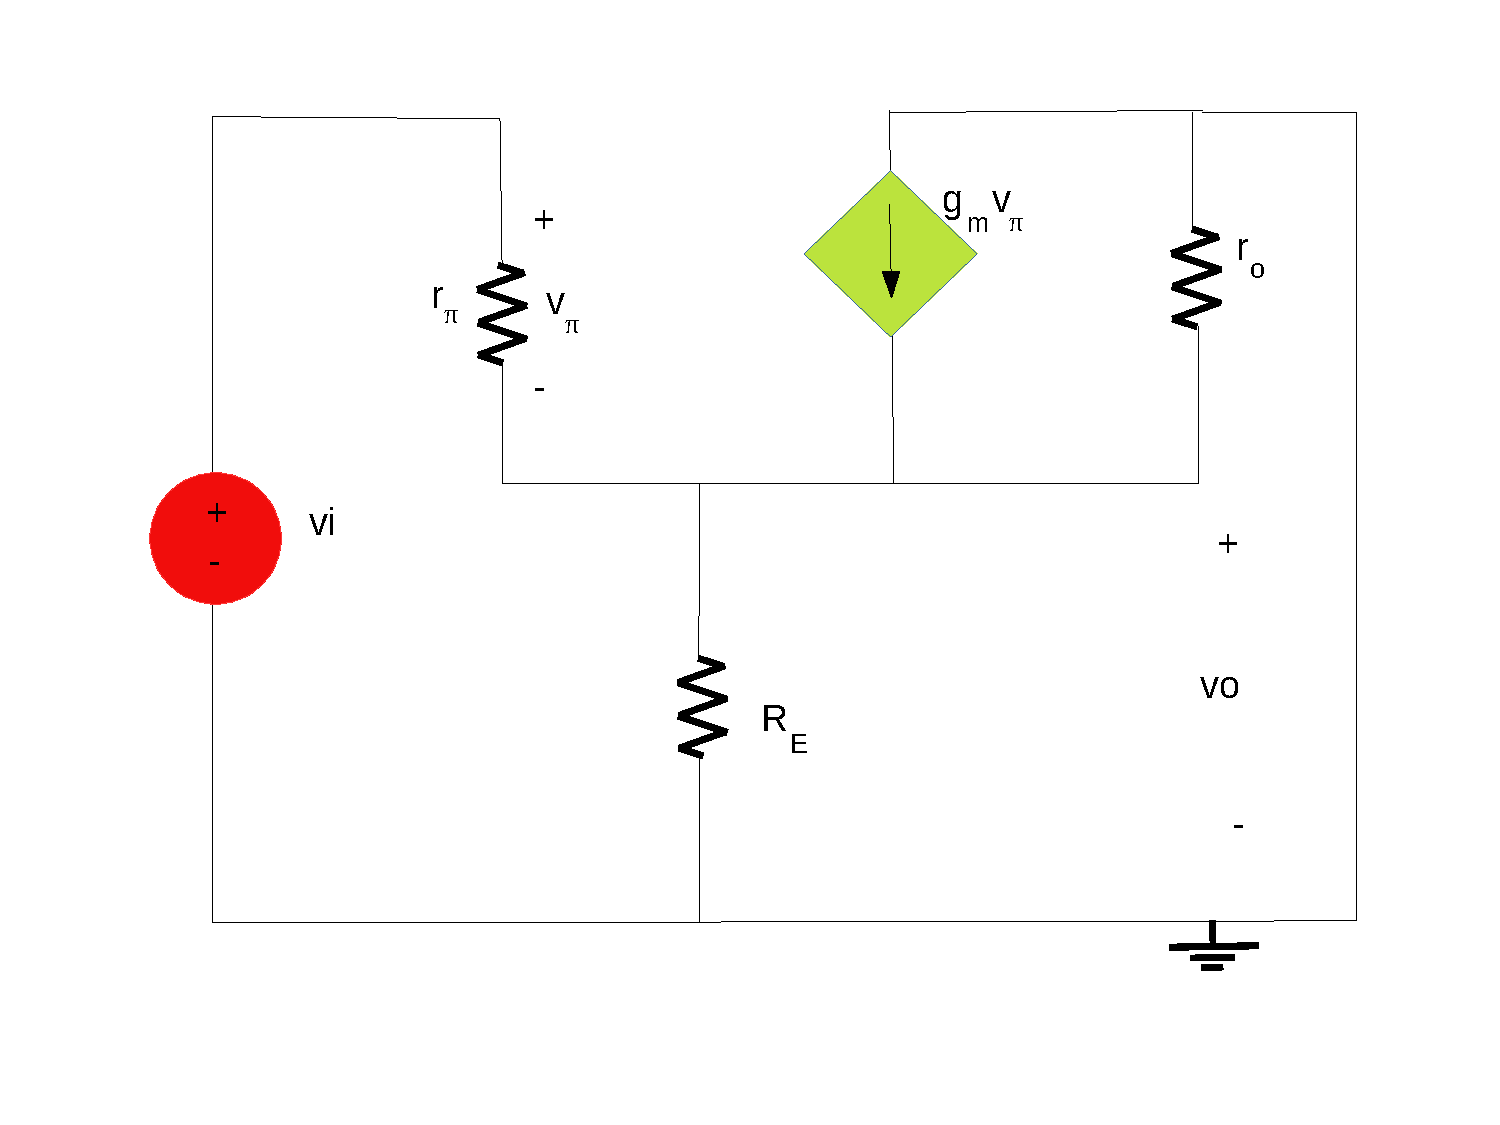
\includegraphics[width=0.5\linewidth]{lab41.pdf}
\caption{Model for the output stage incremental analysis}
\label{s}
\end{figure}


\subsection{Final Results}


Finally, we calculated $i_o$ to then compute $Z_o=\frac{v_{o}}{i_o}=\frac{1}{g_{o2}+g_{m2}\frac{r_{\pi 2}}{r_{\pi 2}+Z_{o1}}+g_{e2}+\frac{1}{r_{\pi 2}+Z_{o1}}}$ using the provided equations. The gain is given by $A_V = A_{V1}*{AV2}$.

We also computed the low cutoff frequency in octave.
All the important results obtained are shown in the tables and in the figure bellow. As we can see, there will not be signal loss since $Z_{i2}>>Z_{o1}$.

\begin{figure}[h] \centering
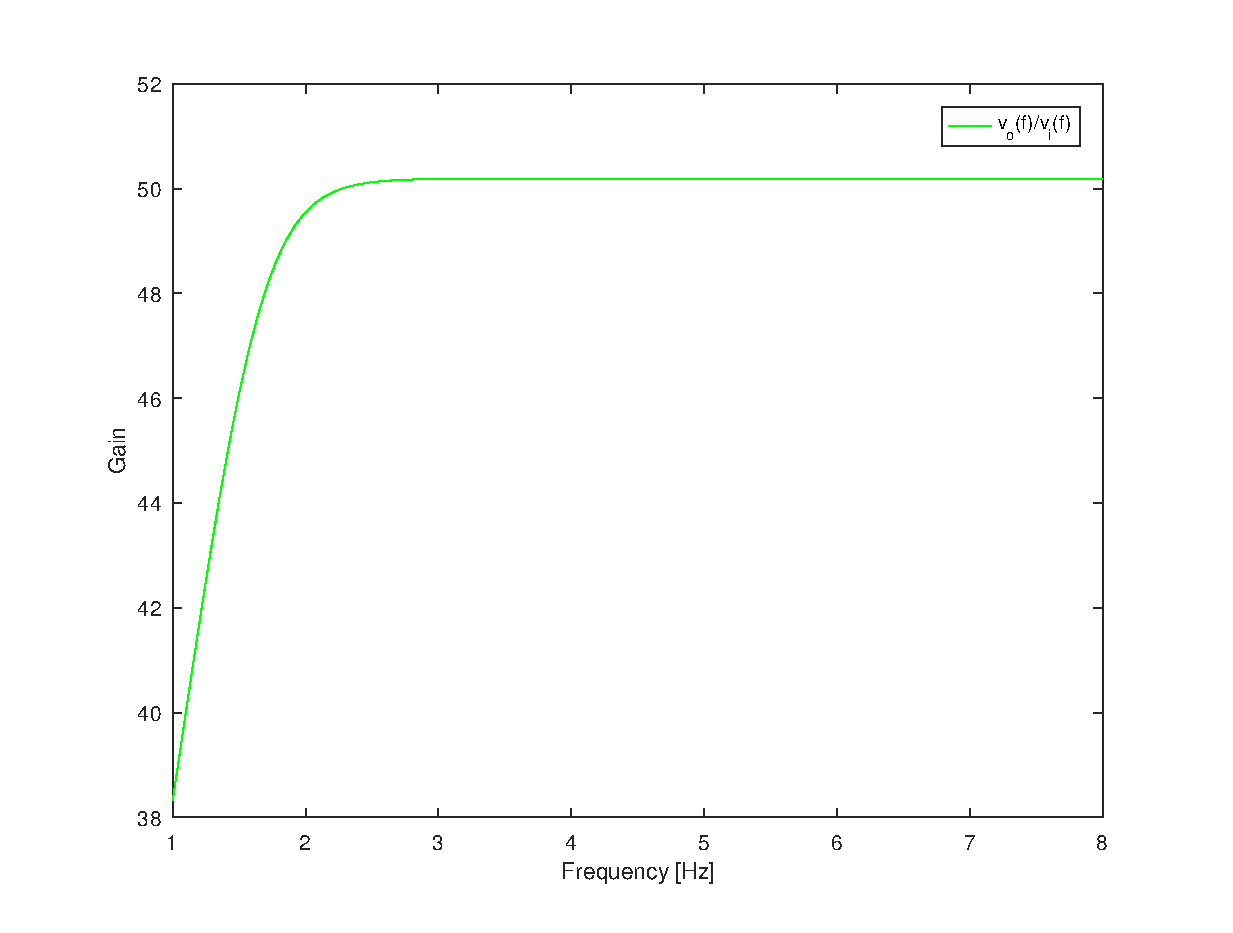
\includegraphics[width=0.65\linewidth]{theo.eps}
\caption{Voltage Gain of the circuit. Octave}
\label{sh}
\end{figure}


\begin{table}[ht]
  \centering
  \begin{tabular}{|l|r|}
    \hline    
    {\bf Name} & {\bf Value} \\ \hline
    IB1 & 1.975467e-05 \\ \hline
IC1 & 3.530160e-03 \\ \hline
IE1 & 3.549915e-03 \\ \hline
VColl & 1.409519e+00 \\ \hline
VBase & 1.090909e+00 \\ \hline
VEmit & 3.549915e-01 \\ \hline

  \end{tabular}
  \caption{Operating point currents and Vcoll.}
  \label{tab:1}
\end{table}


\begin{table}[ht]
  \centering
  \begin{tabular}{|l|r|}
    \hline    
    {\bf Name} & {\bf Value} \\ \hline
    \input{../mat/Z_tab}
  \end{tabular}
  \caption{Impedences of both stages and of the full circuit.}
  \label{tab:2}
\end{table}



\begin{table}[ht]
  \centering
  \begin{tabular}{|l|r|}
    \hline    
    {\bf Name} & {\bf Value} \\ \hline
    Total Gain (AV)  & 3.035752e+02 V\\ \hline
Bandwidth& 1.348349e+06 Hz \\ \hline
Lower Cut Off Frequency& 5.094138e+01 Hz \\ \hline

  \end{tabular}
  \caption{Gain, bandwidth and cutoff frequency.}
  \label{tab:3}
\end{table}












